\documentclass[letterpaper, 11pt]{article}

% --- Package imports ---

\usepackage{
  amsmath, amsthm, amssymb, mathtools, dsfont,	  % Math typesetting
  graphicx, wrapfig, subfig, float,                  % Figures and graphics formatting
  listings, color, inconsolata, pythonhighlight,     % Code formatting
  algorithm,algorithmic,fancyhdr, sectsty, hyperref, enumerate, enumitem } % Headers/footers, section fonts, links, lists

% --- Page layout settings ---

% Set page margins
\usepackage[left=1.35in, right=1.35in, bottom=1in, top=1.1in, headsep=0.2in]{geometry}

% Anchor footnotes to the bottom of the page
\usepackage[bottom]{footmisc}

% Set line spacing
\renewcommand{\baselinestretch}{1.2}

% Set spacing between paragraphs
\setlength{\parskip}{1.5mm}

% Allow multi-line equations to break onto the next page
\allowdisplaybreaks

% Enumerated lists: make numbers flush left, with parentheses around them
\setlist[enumerate]{wide=0pt, leftmargin=21pt, labelwidth=0pt, align=left}
\setenumerate[1]{label={(\arabic*)}}

% --- Page formatting settings ---

% Set link colors for labeled items (blue) and citations (red)
\hypersetup{colorlinks=true, linkcolor=blue, citecolor=red}

% Make reference section title font smaller
\renewcommand{\refname}{\large\bf{References}}

% --- Settings for printing computer code ---

% Define colors for green text (comments), grey text (line numbers),
% and green frame around code
\definecolor{greenText}{rgb}{0.5, 0.7, 0.5}
\definecolor{greyText}{rgb}{0.5, 0.5, 0.5}
\definecolor{codeFrame}{rgb}{0.5, 0.7, 0.5}

% Define code settings
\lstdefinestyle{code} {
  frame=single, rulecolor=\color{codeFrame},            % Include a green frame around the code
  numbers=left,                                         % Include line numbers
  numbersep=8pt,                                        % Add space between line numbers and frame
  numberstyle=\tiny\color{greyText},                    % Line number font size (tiny) and color (grey)
  commentstyle=\color{greenText},                       % Put comments in green text
  basicstyle=\linespread{1.1}\ttfamily\footnotesize,    % Set code line spacing
  keywordstyle=\ttfamily\footnotesize,                  % No special formatting for keywords
  showstringspaces=false,                               % No marks for spaces
  xleftmargin=1.95em,                                   % Align code frame with main text
  framexleftmargin=1.6em,                               % Extend frame left margin to include line numbers
  breaklines=true,                                      % Wrap long lines of code
  postbreak=\mbox{\textcolor{greenText}{$\hookrightarrow$}\space} % Mark wrapped lines with an arrow
}

% Set all code listings to be styled with the above settings
\lstset{style=code}

% --- Math/Statistics commands ---

% Add a reference number to a single line of a multi-line equation
% Usage: "\numberthis\label{labelNameHere}" in an align or gather environment
\newcommand\numberthis{\addtocounter{equation}{1}\tag{\theequation}}

% Shortcut for bold text in math mode, e.g. $\b{X}$
\let\b\mathbf

% Shortcut for bold Greek letters, e.g. $\bg{\beta}$
\let\bg\boldsymbol

% Shortcut for calligraphic script, e.g. %\mc{M}$
\let\mc\mathcal

% \mathscr{(letter here)} is sometimes used to denote vector spaces
\usepackage[mathscr]{euscript}

% Convergence: right arrow with optional text on top
% E.g. $\converge[w]$ for weak convergence
\newcommand{\converge}[1][]{\xrightarrow{#1}}

% Normal distribution: arguments are the mean and variance
% E.g. $\normal{\mu}{\sigma}$
\newcommand{\normal}[2]{\mathcal{N}\left(#1,#2\right)}

% Uniform distribution: arguments are the left and right endpoints
% E.g. $\unif{0}{1}$
\newcommand{\unif}[2]{\text{Uniform}(#1,#2)}

% Independent and identically distributed random variables
% E.g. $ X_1,...,X_n \iid \normal{0}{1}$
\newcommand{\iid}{\stackrel{\smash{\text{iid}}}{\sim}}

% Equality: equals sign with optional text on top
% E.g. $X \equals[d] Y$ for equality in distribution
\newcommand{\equals}[1][]{\stackrel{\smash{#1}}{=}}

% Math mode symbols for common sets and spaces. Example usage: $\R$
\newcommand{\R}{\mathbb{R}}   % Real numbers
\newcommand{\C}{\mathbb{C}}   % Complex numbers
\newcommand{\Q}{\mathbb{Q}}   % Rational numbers
\newcommand{\Z}{\mathbb{Z}}   % Integers
\newcommand{\N}{\mathbb{N}}   % Natural numbers
\newcommand{\F}{\mathcal{F}}  % Calligraphic F for a sigma algebra
\newcommand{\El}{\mathcal{L}} % Calligraphic L, e.g. for L^p spaces

% Math mode symbols for probability
\newcommand{\pr}{\mathbb{P}}    % Probability measure
\newcommand{\E}{\mathbb{E}}     % Expectation, e.g. $\E(X)$
\newcommand{\var}{\text{Var}}   % Variance, e.g. $\var(X)$
\newcommand{\cov}{\text{Cov}}   % Covariance, e.g. $\cov(X,Y)$
\newcommand{\corr}{\text{Corr}} % Correlation, e.g. $\corr(X,Y)$
\newcommand{\B}{\mathcal{B}}    % Borel sigma-algebra

% Other miscellaneous symbols
\newcommand{\tth}{\text{th}}	% Non-italicized 'th', e.g. $n^\tth$
\newcommand{\Oh}{\mathcal{O}}	% Big-O notation, e.g. $\O(n)$
\newcommand{\1}{\mathds{1}}	% Indicator function, e.g. $\1_A$

% Additional commands for math mode
\DeclareMathOperator*{\argmax}{argmax}    % Argmax, e.g. $\argmax_{x\in[0,1]} f(x)$
\DeclareMathOperator*{\argmin}{argmin}    % Argmin, e.g. $\argmin_{x\in[0,1]} f(x)$
\DeclareMathOperator*{\spann}{Span}       % Span, e.g. $\spann\{X_1,...,X_n\}$
\DeclareMathOperator*{\bias}{Bias}        % Bias, e.g. $\bias(\hat\theta)$
\DeclareMathOperator*{\ran}{ran}          % Range of an operator, e.g. $\ran(T) 
\DeclareMathOperator*{\dv}{d\!}           % Non-italicized 'with respect to', e.g. $\int f(x) \dv x$
\DeclareMathOperator*{\diag}{diag}        % Diagonal of a matrix, e.g. $\diag(M)$
\DeclareMathOperator*{\trace}{trace}      % Trace of a matrix, e.g. $\trace(M)$

% Numbered theorem, lemma, etc. settings - e.g., a definition, lemma, and theorem appearing in that 
% order in Section 2 will be numbered Definition 2.1, Lemma 2.2, Theorem 2.3. 
% Example usage: \begin{theorem}[Name of theorem] Theorem statement \end{theorem}
\theoremstyle{definition}
\newtheorem{theorem}{Theorem}[section]
\newtheorem{proposition}[theorem]{Proposition}
\newtheorem{lemma}[theorem]{Lemma}
\newtheorem{corollary}[theorem]{Corollary}
\newtheorem{definition}[theorem]{Definition}
\newtheorem{example}[theorem]{Example}
\newtheorem{remark}[theorem]{Remark}

% Un-numbered theorem, lemma, etc. settings
% Example usage: \begin{lemma*}[Name of lemma] Lemma statement \end{lemma*}
\newtheorem*{theorem*}{Theorem}
\newtheorem*{proposition*}{Proposition}
\newtheorem*{lemma*}{Lemma}
\newtheorem*{corollary*}{Corollary}
\newtheorem*{definition*}{Definition}
\newtheorem*{example*}{Example}
\newtheorem*{remark*}{Remark}
\newtheorem*{claim}{Claim}

% --- Left/right header text (to appear on every page) ---

% Include a line underneath the header, no footer line
\pagestyle{fancy}
\renewcommand{\footrulewidth}{0pt}
\renewcommand{\headrulewidth}{0.4pt}
\newcommand{\homework}[1]{
   \pagestyle{myheadings}
   \thispagestyle{plain}
   \newpage
   \setcounter{page}{1}
   \noindent
   \classname \hfill \mbox{Updated Day Here} \\
   \instname \hfill \mbox{\duedate}
   \rule{6.5in}{0.5mm}
   \vspace*{-0.1 in}
}
\usepackage{pgf,tikz}
\usetikzlibrary{shapes,arrows,automata}

\usepackage{listings}
\usepackage{xcolor}
\lstset { %
    language=C++,
    backgroundcolor=\color{black!5}, % set backgroundcolor
    basicstyle=\footnotesize,% basic font setting
}


\newcommand{\problem}[1]{\section*{Problem #1}}


\renewcommand{\labelenumi}{(\alph{enumi})}
\renewcommand{\labelenumii}{(\roman{enumii})}
\newenvironment{solution}{{\par\noindent\it Solution.}}{}
% Left header text: course name/assignment number
\lhead{CSCI-SHU 220: Algorithms\\Homework 3}

% Right header text: your name
\rhead{Posted: March 28, 2025\\Due: 11:55pm (Shanghai time), April 17, 2025}

% --- Document starts here ---

\begin{document}

This assignment has in total $100$ base points and $10$ extra points, and the cap is $100$.
Bonus questions are indicated using the $\star$ mark.

Submission Instructions: Please submit to Gradescope. During submission, you need to \textbf{mark/map the solution to each question}; otherwise, we may apply a penalty. 

Another notice: you only get full credits for the algorithm design questions if your algorithm matches the desirable complexity. If the desirable complexity is not stated, you need to design an algorithm to be as fast as possible.

\textit{Please specify the following information before submission}:
\begin{itemize}
    \item Your Name: Yixia Yu%  (put your name here)
    \item Your NetID: yy5091 % (put your NetID here)
\end{itemize}
\clearpage

\problem{1: Infinite Knapsack [$10^\star+15$ pts]}
Recall that in the infinite knapsack problem, we are given a knapsack with capacity $W$ and $m$ types of (infinite) items $I_1,\dots,I_m$, where $I_i$ has weight $w_i \in \mathbb{N}$ and value $v_i \in \mathbb{R}_{>0}$.
Our goal is to include in the knapsack items of total weight at most $W$ with maximum total value.
Formally, we want to compute $m$ non-negative integers $n_1,\dots,n_m$ satisfying $\sum_{i=1}^m n_i w_i \leq W$ such that $\sum_{i=1}^m n_i v_i$ is maximized (here $n_i$ indicates the number of copies of $I_i$ included in the knapsack).
In the lecture, we have already seen that this problem can be solved in $O(mW)$ time.
In this exercise, we try to design another algorithm with running time $O(mw_{\max}^2)$ where $w_{\max} = \max_{i=1}^m w_i$.
This task is somehow challenging.
So we divide it into the following two steps.
Also, for simplicity, we assume that the value-weight ratios of the items are distinct and sorted, i.e., $\frac{v_1}{w_1} > \frac{v_2}{w_2} > \cdots > \frac{v_m}{w_m}$.

\begin{enumerate}
    \item[(a)$^\star$] Prove that in any optimal solution $(n_1,\dots,n_m)$, the total number of copies of the items $I_2,\dots,I_m$ included in the knapsack is at most $w_{\max}-1$, i.e., $\sum_{i=2}^m n_i \leq w_{\max}-1$.
    \item[(b)] Based on the conclusion of (a), design an algorithm $\textsc{Knapsack}(m,W,(w_1,v_1),\dots,(w_m,v_m))$ for infinite knapsack with running time $O(mw_{\max}^2)$.
    For convenience, your algorithm only need to return the maximum value achieved.
    Describe the basic idea and give the pseudocode.
    Briefly justify the correctness and analyze the time complexity. \\[1ex]
    (\textbf{Hint:} According to (a), we know that, in an optimal solution, the total \textit{weight} of the items $I_2,\dots,I_m$ is $O(w_{\max}^2)$, and hence the item $I_1$ occupies ``most'' space of the knapsack. Try to combine this observation with the $O(mW)$-time DP algorithm.)
\end{enumerate}
\begin{solution}
(a):
Assume for contradiction that there is an optimal solution with
\[
\sum_{i=2}^m n_i \ge w_{\max} \geq w_1.
\]
Since each item has weight at least \(1\), the items \(I_2,\dots,I_m\) contribute a total weight of at least \(w_{\max}\). But item \(I_1\) has the highest value-to-weight ratio:
\[
\frac{v_1}{w_1}>\frac{v_i}{w_i}\quad\text{for all } i\ge 2.
\]
Thus, by replacing some copies among \(I_2,\dots,I_m\) that amount to a total weight of (at least) \(w_1\) with one copy of \(I_1\), we would obtain a strictly higher total value, contradicting the optimality. Hence, 
\[
\sum_{i=2}^m n_i\le w_{\max}-1.
\]
(b):
Define a function \(g(x)\) for \(0\le x\le w_{\max}^2\) as the maximum total value achievable by using items \(I_2,\dots,I_m\) with total weight exactly \(x\). Since the total number of copies used from \(I_2,\dots,I_m\) is at most \(w_{\max}-1\), we only need to consider at most \(w_{\max}-1\) copies per item.

For each item \(I_i\) (\(i=2,\dots,m\)) and for each possible copy count \(k\) (with \(0\le k\le w_{\max}-1\), provided that \(x + k\,w_i \le w_{\max}^2\)), update the DP as follows:
\[
g(x+k\,w_i) = \max\{ g(x+k\,w_i),\ g(x) + k\,v_i \}.
\]
Since the state space is up to \(w_{\max}^2\) and we process \(m-1\) items, the overall time for this DP is \(O(mw_{\max}^2)\).


For each weight \(x\) (with \(0\le x\le \min(w_{\max}^2,\,W)\)) achievable by items \(I_2,\dots,I_m\), the remaining capacity is \(W-x\). Since \(I_1\) is the most efficient, we fill the remaining capacity with as many copies of \(I_1\) as possible:
\[
n_1 = \left\lfloor \frac{W-x}{w_1} \right\rfloor,
\]
contributing a value of
\[
n_1\cdot v_1.
\]
Thus, for each \(x\) we compute the overall value:
\[
V(x) = g(x) + \left\lfloor \frac{W-x}{w_1} \right\rfloor v_1.
\]
We then choose the \(x\) maximizing \(V(x)\).
\begin{lstlisting}
    def infinite_knapsack(m, W, items):
        w1, v1 = items[0]
        w_max = max(w for w, v in items)
        maxX = min(W, (w_max - 1) * w_max)
        
        g = [-float('inf')] * (maxX + 1)
        g[0] = 0
        
        for i in range(1, m):
            wi, vi = items[i]
            for x in range(maxX + 1):
                if g[x] != -float('inf'):
                    k = 1
                    while x + k * wi <= maxX:
                        g[x + k * wi] = max(g[x + k * wi], g[x] + k * vi)
                        k += 1
                        
        ans = 0
        for x in range(min(maxX, W) + 1):
            copies = (W - x) // w1
            ans = max(ans, g[x] + copies * v1)
            
        return ans
    \end{lstlisting}
    
\subsection*{Complexity}

The DP runs in \(O(mw_{\max}^2)\) time, and the final evaluation over the \(w_{\max}^2\) states takes an additional \(O(w_{\max}^2)\) time. Therefore, the total running time is \(O(mw_{\max}^2)\).

\end{solution}

\clearpage

\problem{2: Counting Shortest Paths [$15$ pts]}
Given an undirected graph $G = (V,E)$ and a vertex $s \in V$, we want to know for every vertex $t \in V$, how many (distinct) shortest paths from $s$ to $t$ there are.
This can be viewed as a generalization of the unique shortest-path problem.
Design an algorithm $\textsc{Count}(G,s)$ to solve this problem.
The algorithm should return a list $L$ that contains a pair $(v,\delta_v)$ for each vertex $v$ of $G$, where $\delta_v$ is the number of shortest paths from $s$ to $v$.
Describe the basic idea and give the pseudocode.
Briefly justify the correctness and analyze the time complexity.
Your algorithm should run in $O(n+m)$ time, where $n = |V|$ and $m = |E|$.

\textbf{A sample example.}
Suppose the input graph is $G = (V,E)$ where $V = \{s,a,b,c,d,e\}$ and $E = \{(a,b),(b,c),(c,d),(a,d),(s,a),(c,e)\}$; see the figure below.
Then the algorithm $\textsc{Count}(G,s)$ should return $L = [(s,1),(a,1),(b,1),(c,2),(d,1),(e,2)]$.

(\textbf{Hint:} Exploit the BFS tree and extend the idea in the unique shortest-path problem.)

\begin{center}
    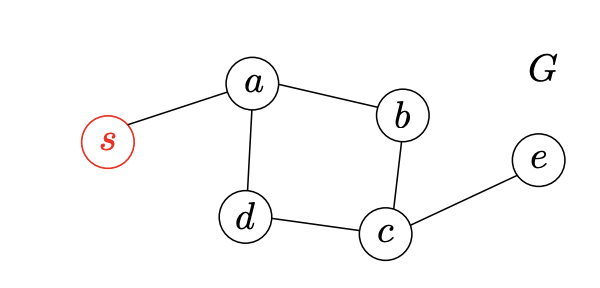
\includegraphics[height=3cm]{1.png}
\end{center}

\begin{solution}
    We extend the standard BFS algorithm to compute the number of distinct shortest paths from a given source vertex \(s\) to every vertex in an undirected graph \(G = (V,E)\). The key idea is to maintain an additional array, \(\mathtt{count}\), where \(\mathtt{count}[v]\) stores the number of shortest paths from \(s\) to vertex \(v\).

    The process is as follows:
    \begin{itemize}
        \item Initialize \(\mathtt{count}[s] = 1\), because there is exactly one path from \(s\) to itself.
        \item When exploring a vertex \(v\) during the BFS, for each neighbor \(u\) of \(v\):
        \begin{itemize}
            \item If \(u\) is discovered for the first time, set
            \[
            \mathtt{count}[u] \gets \mathtt{count}[v],
            \]
            and record that \(\texttt{dist}[u] = \texttt{dist}[v] + 1\).
            \item If \(u\) has been discovered previously and the current edge leads to a shortest path, i.e., if
            \[
            \texttt{dist}[u] = \texttt{dist}[v] + 1,
            \]
            then update
            \[
            \mathtt{count}[u] \gets \mathtt{count}[u] + \mathtt{count}[v].
            \]
        \end{itemize}
    \end{itemize}
    
    In this way, all shortest paths reaching a vertex \(u\) from different preceding vertices are accumulated into \(\mathtt{count}[u]\).
\begin{lstlisting}
    Count(G, s)
    visited[v] ← False for all v ∈ V
    Q[0] ← s and visited[s] ← True
    dist[s] ← 0, count[s] ← 1 and pred[s] ← Null 
    head, tail ← 0
    while head ≤ tail do
        v ← Q[head]
        for every neighbor u of v do
            if visited[u] = False then
                tail ← tail + 1
                Q[tail] ← u and visited[u] ← True
                dist[u] ← dist[v] + 1
                count[u] ← count[v]        
                pred[u] ← v
            else if dist[u] = dist[v] + 1 then
                count[u] ← count[u] + count[v] 
            end if
        end for
        head ← head + 1
    end while
    return L = { (v, count[v]) for all v in V }
\end{lstlisting}
\section*{Correctness}

The algorithm extends BFS, which processes vertices in non-decreasing order of their distance from the source \(s\). When a vertex \(u\) is discovered for the first time through a vertex \(v\), we set 
\[
\texttt{dist}[u] = \texttt{dist}[v] + 1 \quad \text{and} \quad \texttt{count}[u] = \texttt{count}[v].
\]
If \(u\) is encountered again via another predecessor \(w\) such that 
\[
\texttt{dist}[w] + 1 = \texttt{dist}[u],
\]
the algorithm adds \(\texttt{count}[w]\) to \(\texttt{count}[u]\). This ensures that all shortest paths leading to \(u\) are counted, as each shortest path to \(u\) must come from a vertex in the previous layer.

\section*{Time Complexity}

The algorithm is based on BFS, where:
\begin{itemize}
    \item Each vertex is enqueued and processed exactly once.
    \item Each edge is examined at most once.
\end{itemize}
Thus, the overall time complexity is \(O(n + m)\), where \(n = |V|\) and \(m = |E|\).
\end{solution}
\clearpage

\problem{3: Reaching the One [$15$ pts]}
Let $n \geq 3$ be a given positive integer and we are going to play a game as follows.
During the game, we have a number $k$ which is initially equal to $2$.
In each round of the game, we are allowed to change the current number $k$ to a new number in one of the following ways:
\begin{itemize}
    \item \textbf{Type-A:} Change $k$ to $(k+1) \text{ mod } n$.
    \item \textbf{Type-B:} Change $k$ to a divisor of $k$ that is greater than $1$.
    \item \textbf{Type-C:} Change $k$ to $k^2 \text{ mod } n$.
\end{itemize}

Note that the above three rules guarantee that our number $k$ is always in the range $\{0,1,\dots,n-1\}$ during the entire game.
The game terminates when $k$ becomes $1$.
Our goal is to finish the game in \textit{fewest} rounds.
For example, suppose $n = 91$ and we can play the game as follows.
\begin{itemize}
    \item \textbf{Round 1:} $2 \Longrightarrow 3$ using Type-A change.
    \item \textbf{Round 2:} $3 \Longrightarrow 9$ using Type-C change.    
    \item \textbf{Round 3:} $9 \Longrightarrow 81$ using Type-C change.
    \item \textbf{Round 4:} $81 \Longrightarrow 27$ using Type-B change.
    \item \textbf{Round 5:} $27 \Longrightarrow 1$ using Type-C change.    
\end{itemize}
As you can verify, this is an optimal solution.
Design an algorithm $\textsc{Game}(n)$ which returns an optimal solution to the game as a list.
So $\textsc{Game}(91)$ should return $[2,3,9,81,27,1]$ (or another solution with $5$ rounds).
Describe the basic idea and give the pseudocode.
Briefly justify the correctness and analyze the time complexity.
Your algorithm should run in $O(n \log n)$ time.

(\textbf{Hint:} Formulate the problem as a graph problem with $n$ vertices and $O(n \log n)$ edges.)

\begin{solution}
    We transform the game into a shortest-path problem on a directed graph where each vertex represents a state \( k \) in the set \(\{0, 1, 2, \dots, n-1\}\). The allowed moves form the edges of the graph:
    \begin{itemize}
        \item \textbf{Type-A:} There is an edge from \( k \) to \((k+1) \mod n\).
        \item \textbf{Type-C:} There is an edge from \( k \) to \( k^2 \mod n\).
        \item \textbf{Type-B:} For every divisor \( d \) of \( k \) with \( d > 1 \), there is an edge from \( k \) to \( d \).
    \end{itemize}
    The game starts at vertex \(2\) and terminates when we reach vertex \(1\). Since every move has a unit cost, finding the shortest path from \(2\) to \(1\) in this graph yields an optimal solution in terms of the minimum number of rounds.
    
    To efficiently generate Type-B edges, we preprocess the divisors for each \( k \) in \( O(n \log n) \) time (using a sieve-like method). After this preprocessing, a standard breadth-first search (BFS) is used to traverse the graph, keep track of distance (number of rounds), and record predecessor information to reconstruct the optimal sequence of moves.
\begin{lstlisting}
    Game(n)
    for k from 0 to n-1 do
        D[k] ← [] 
    for d from 2 to n-1 do
        for multiple k = d, 2d, 3d, …, while k < n do
            Append d to D[k]
    visited[v] ← False for all v in {0,1,..., n-1}
    dist[v] ← ∞ for all v in {0,1,..., n-1}
    pred[v] ← Null for all v in {0,1,..., n-1}
    Q[0] ← 2 and visited[2] ← True
    dist[2] ← 0
    head, tail ← 0
    while head ≤ tail do
        v ← Q[head]
        if v = 1 then
            break  
        u_A ← (v + 1) mod n
        if visited[u_A] = False then
            tail ← tail + 1
            Q[tail] ← u_A
            visited[u_A] ← True
            dist[u_A] ← dist[v] + 1
            pred[u_A] ← v
        u_C ← (v * v) mod n
        if visited[u_C] = False then
            tail ← tail + 1
            Q[tail] ← u_C
            visited[u_C] ← True
            dist[u_C] ← dist[v] + 1
            pred[u_C] ← v
        for each u_B in D[v] do
            if visited[u_B] = False then
                tail ← tail + 1
                Q[tail] ← u_B
                visited[u_B] ← True
                dist[u_B] ← dist[v] + 1
                pred[u_B] ← v
        head ← head + 1
    if visited[1] = False then
        return "No valid solution"  
    else
        path ← []
        curr ← 1
        while curr ≠ Null do
            Prepend curr to path
            curr ← pred[curr]
        return path
\end{lstlisting}
\section*{Correctness Analysis}

\begin{itemize}
    \item  Every allowed move in the game is correctly represented by an edge in the graph. Therefore any sequence of moves corresponds to a path in the graph.
    \item  Since BFS processes vertices in layers (non-decreasing order of distance from the source), the first time the vertex \(1\) is encountered, it is guaranteed to be reached via the shortest path (i.e., the fewest moves).
    \item The predecessor pointers maintained during BFS allow us to reconstruct the sequence of moves, ensuring that the returned solution is optimal.
\end{itemize}

\section*{Time Complexity Analysis}

 The BFS visits each vertex at most once. Besides the constant-time Type-A and Type-C moves for each vertex, the Type-B moves add edges in number proportional to the number of divisors, which on average is \(O(\log n)\). Hence, the total number of edges examined is \(O(n \log n)\). This leads to a BFS time complexity of \( O(n \log n) \).


Thus, the algorithm runs in \( O(n \log n) \) time.

\end{solution}
\clearpage

\problem{4: Finding a Strongly Connected Component [$10$ pts]}
Given a \textit{directed} graph $G = (V,E)$ and a vertex $s \in V$, we want to compute the strongly connected component of $G$ containing $s$.
Design an algorithm $\textsc{SCC}(G,s)$ which returns the set of vertices of $G$ that lie in the same strongly connected component as $s$.
Describe the basic idea and give the pseudocode.
Briefly justify the correctness and analyze the time complexity.
Your algorithm should run in $O(n+m)$ time, where $n = |V|$ and $m = |E|$.

(\textbf{Hint:} By definition, a vertex $v$ is in the same strongly connected component as $s$ iff $v$ is reachable from $s$ and $s$ is reachable from $v$. We already know how to find the vertices reachable from $s$ using DFS. Can you use a similar idea to compute the vertices from which $s$ is reachable?)

\begin{solution}
By definition, a vertex \(v\) is in the same SCC as \(s\) if and only if:
\[
s \rightarrow v \quad \text{and} \quad v \rightarrow s,
\]
meaning that \(s\) can reach \(v\) and \(v\) can reach \(s\).

The algorithm employs the following steps:
\begin{enumerate}
    \item \textbf{Forward DFS:} Run a Depth First Search (DFS) on the original graph \(G\) starting from \(s\). Let \(R\) be the set of vertices that are reachable from \(s\). This ensures that for every vertex \(v \in R\), the path \(s \rightarrow v\) exists.
    \item \textbf{Construct the Reverse Graph:} Create a new graph \(G_{\text{rev}}\) by reversing the direction of every edge in \(G\). Specifically, for every edge \((u, v) \in E\), add the edge \((v, u)\) to \(G_{\text{rev}}\).
    \item \textbf{Reverse DFS:} Run a DFS on \(G_{\text{rev}}\) starting from \(s\). Let \(R_{\text{rev}}\) be the set of vertices reachable from \(s\) in \(G_{\text{rev}}\). In the original graph \(G\), this corresponds to all vertices that can reach \(s\) (i.e., \(v \rightarrow s\)).
    \item \textbf{Intersection:} The strongly connected component containing \(s\) is given by:
    \[
    \text{SCC}(s) = R \cap R_{\text{rev}}.
    \]
\end{enumerate}
\begin{lstlisting}
    Algorithm SCC(G, s)
    Input: Directed graph G = (V, E), vertex s in V
    Output: The set of vertices in the same SCC as s
    R = DFS(G, s)
    G_rev = ReverseGraph(G)
    R_rev = DFS(G_rev, s)
    return R ∩ R_rev

Function DFS(G, s):
    Initialize visited[v] = false for each v in V
    Initialize result = empty set
    DFS_Visit(s)
    
    Procedure DFS_Visit(v):
        visited[v] = true
        add v to result
        for each neighbor u of v in G:
            if visited[u] == false:
                DFS_Visit(u)
                
    return result

Function ReverseGraph(G):
    Create a new graph G_rev with vertices V and an empty set of edges
    for each edge (u, v) in E:
        add edge (v, u) to G_rev
    return G_rev
\end{lstlisting}
\section*{Correctness Analysis}

The forward DFS guarantees that all vertices reachable from \(s\) (the \(s \rightarrow v\) condition) are included in \(R\). Meanwhile, after constructing the reverse graph \(G_{\text{rev}}\), running DFS from \(s\) finds all vertices that have a path from them to \(s\) in the original graph (because in \(G_{\text{rev}}\), the paths are reversed). The intersection \(R \cap R_{\text{rev}}\) appropriately narrows the search to exactly those vertices satisfying both properties. Hence, the procedure correctly identifies the SCC containing \(s\).

\section*{Time Complexity Analysis}

\begin{itemize}
    \item The forward DFS on \(G\) takes \(O(n+m)\), where \(n=|V|\) and \(m=|E|\).
    \item Constructing the reverse graph \(G_{\text{rev}}\) requires processing each edge once, which takes \(O(m)\) time.
    \item The DFS on \(G_{\text{rev}}\) similarly takes \(O(n+m)\).
    \item The intersection operation \(R \cap R_{\text{rev}}\) can be performed in \(O(n)\) time, assuming efficient set membership checks.
\end{itemize}

Overall, the algorithm runs in:
\[
O(n+m) + O(m) + O(n+m) + O(n) = O(n+m)
\]
Thus, the entire process has a time complexity of \(O(n+m)\).

\end{solution}
\clearpage



\problem{5: Construct a Party [$15$ pts]}
We want to organize a party involving $n$ couples. We have to invite exactly one person from each couple. Also, for every person, it has a list of friends in the $n$ couples that also need to be invited, or otherwise that person will not come. Another ``social norm'' we observe is that for a couple $(x, y)$,  if $x$ wants to invite a friend $x'$ from a couple, the partner of $x'$ will also invite $y$

\begin{enumerate}
    \item Build a graph with $2n$ nodes (the $2n$ people in $n$ couples). Add an edge $(a,b)$ if $a$ would come only if you also invite $b$. This gives a graph $G$. Prove that if a couple is in the same strongly connected component of $G$, then you can not organize a valid party.

    \item Prove the converse of the previous subquestion. I.e., if no strongly connected component in $G$ contains a couple, then there are $n$ invitations that would result in a valid party.

    \item Provide a linear algorithm (in terms of the size of $G$) to compute if there is a valid party as well as generating the invitations if valid.
\end{enumerate}

\begin{solution}
(1) We build a directed graph \( G = (V, E) \) where the vertex set \( V \) consists of all \( 2n \) individuals. If a couple $(X,Y)$ is in the same strongly connected component of $G$, then by definition there exist directed paths
\[
x \rightarrow \cdots \rightarrow y \quad \text{and} \quad y \rightarrow \cdots \rightarrow x.
\]
These paths imply that if \( x \) is invited, then by following the dependency edges along \( x \rightarrow \cdots \rightarrow y \), the party must also include \( y \). Likewise, if \( y \) is invited, then following the path \( y \rightarrow \cdots \rightarrow x \) forces the inclusion of \( x \).
\\(2)
We model each couple $(x_i,y_i)$ by two literals $x_i,\;\bar x_i=y_i$ and build a directed graph $G=(V,E)$ as follows:
\begin{align*}
&V=\{\,x_i,\bar x_i: i=1,\dots,n\},\\
&\text{whenever person }p\text{ requires friend }q\text{ we add}
  \quad p\to q\quad\text{and}\quad \bar q\to\bar p
  \;\in E.
\end{align*}
By hypothesis no couple’s two literals lie in the same strongly‐connected component (SCC).  Let
\[
  C(\ell)\;=\;\text{the index of the SCC containing literal }\ell
\]
in some topological ordering of the condensation of $G$.  Note that
\[
  \ell\to\ell'\;\Longrightarrow\;C(\ell)\;\le\;C(\ell'),
  \quad
  \bar\ell'\to\bar\ell\;\Longrightarrow\;C(\bar\ell')\;\le\;C(\bar\ell).
\]
We now define an invitation‐assignment
\[
  \text{invite}(\ell)
  \;=\;
  \begin{cases}
    \mathrm{True},&C(\ell)>C(\bar\ell),\\
    \mathrm{False},&C(\ell)<C(\bar\ell).
  \end{cases}
\]
Then:
\begin{itemize}
  \item Since $C(\ell)\neq C(\bar\ell)$, exactly one of each couple is invited.
  \item If $\ell\to\ell'$ is an edge and invite$(\ell)=\mathrm{True}$, then
    \[
      C(\ell)>C(\bar\ell)
      \quad\text{and}\quad
      C(\ell)\le C(\ell')
      \quad\Longrightarrow\quad
      C(\ell')>C(\bar\ell).
    \]
    But also $\bar\ell'\to\bar\ell$ gives 
    $C(\bar\ell')\le C(\bar\ell)<C(\ell')$, 
    so indeed $C(\ell')>C(\bar\ell')$, i.e.\ invite$(\ell')=\mathrm{True}$.
\end{itemize}
Hence every “if you invite $p$ then you must invite $q$” is satisfied, and by construction each couple contributes exactly one guest.  This completes the proof.
\\(3)
\begin{lstlisting}
    function VALID_PARTY(G, couples)
    for each v in G.vertices
        index[v] ← -1
        onStack[v] ← false
    indexCounter ← 0
    compCount ← 0
    stack ← empty stack
    for each v in G.vertices
        if index[v] < 0
            STRONGCONNECT(v)
    for each (x,y) in couples
        if comp[x] = comp[y]
            return INVALID
    for each v in G.vertices
        invite[v] ← (comp[v] > comp[NOT(v)])
    result ← empty list
    for each (x,y) in couples
        if invite[x]
            append x to result
        else
            append y to result
    return VALID, result

procedure STRONGCONNECT(v)
    index[v] ← indexCounter
    lowlink[v] ← indexCounter
    indexCounter ← indexCounter + 1
    push v onto stack
    onStack[v] ← true
    for each w in G.adj[v]
        if index[w] < 0
            STRONGCONNECT(w)
            lowlink[v] ← min(lowlink[v], lowlink[w])
        else if onStack[w]
            lowlink[v] ← min(lowlink[v], index[w])
    if lowlink[v] = index[v]
        repeat
            w ← pop from stack
            onStack[w] ← false
            comp[w] ← compCount
        until w = v
        compCount ← compCount + 1
\end{lstlisting}
\end{solution}
\clearpage



\problem{6: Nearly Strongly Connected [$10$ pts]}
Given a DAG $G$, we call it ``nearly strongly connected'' if we can flip one edge in $G$ and it becomes strongly connected.

\begin{enumerate}
    \item Prove that $G$ has only one source (node with only outgoing edges) and one sink (node with only incoming edges).
    \item Give one sentence precise description for the edge that should be flipped. Also prove the description is correct.
    \item Give a linear time algorithm (in terms of the size of $G$) for computing the edge of flipping.
\end{enumerate}
\begin{solution}
(1)
Flipping the arc \(u\to v\) into \(v\to u\) removes exactly the edge \(u\to v\) and adds exactly the edge \(v\to u\).  Hence the change in the number of edges entering or leaving each vertex is
\begin{align*}
\Delta\bigl(\text{edges entering }u\bigr)&=+1, 
&\Delta\bigl(\text{edges leaving }u\bigr)&=-1,\\
\Delta\bigl(\text{edges entering }v\bigr)&=-1, 
&\Delta\bigl(\text{edges leaving }v\bigr)&=+1,\\
\Delta\bigl(\text{edges entering or leaving any other }w\bigr)&=0.
\end{align*}
In particular, at most one vertex can gain an entering edge and at most one can gain a leaving edge.

Now suppose, for the sake of contradiction, that \(G\) has two distinct sources \(s_1\) and \(s_2\), i.e.\ no edge enters either \(s_1\) or \(s_2\).  After flipping one arc, at most one of \(\{s_1,s_2\}\) can gain an entering edge, so the other still has none.  But a strongly connected digraph has every vertex reachable from every other, which forces every vertex to have at least one entering edge.  This contradiction shows \(G\) has exactly one source.

Dually, if \(G\) had two distinct sinks \(t_1,t_2\) (no edge leaves them), then flipping a single arc could give an extra leaving edge to at most one, leaving the other without any.  Again this contradicts strong connectivity.  Therefore \(G\) has exactly one sink.
The dual argument applies to sinks (vertices of out‐degree 0): if there were two distinct sinks, flipping a single edge could at best increase the out‐degree of one of them, leaving the other with out‐degree 0 in \(H\), again contradicting strong connectivity.  Therefore \(G\) has exactly one sink as well.
\\(2)
Let \(G\) be a nearly strongly‐connected DAG, and let \(s\) and \(t\) be its unique source and unique sink, then the  only edge whose reversal makes \(G\) strongly connected is the arc \(s\to t\).
\\\emph{(Correctness.)}  
Suppose flipping some arc \(u\to v\) in \(G\) produces a strongly connected graph \(H\).  In \(H\) there must be a directed path from \(t\) to \(s\).  The only new arc in passing from \(G\) to \(H\) is \(v\to u\), so that path must traverse \(v\to u\).  Hence in \(G\) there was already a path \(t\rightsquigarrow v\) and a path \(u\rightsquigarrow s\).  But \(t\) is the unique sink of the DAG \(G\), so it has no outgoing edges and thus cannot reach any vertex except itself; therefore \(v=t\).  Dually, \(s\) is the unique source, so it has no incoming edges and hence no vertex can reach \(s\) except itself; therefore \(u=s\).  Thus the only possible arc to reverse is \(s\to t\).

Conversely,  let H be obtained by reversing \(s\to t\). Since \(s\) is the unique source, it reaches every vertex in \(G\), and since \(t\) is the unique sink, every vertex in \(G\) reaches \(t\).  After reversing \(s\to t\) into \(t\to s\), for any two vertices \(x,y\) we have
\[
  x \;\rightsquigarrow\; t \;\longrightarrow\; s \;\rightsquigarrow\; y
\]
in \(H\), so \(H\) is strongly connected.
\\(3)
\begin{lstlisting}
    FindFlipEdge(G)
        for all v in V
            inDeg[v] ← 0
            outDeg[v] ← 0
        for all (u → v) in E
            outDeg[u] ← outDeg[u] + 1
            inDeg[v] ← inDeg[v] + 1
        sources ← 0, sinks ← 0
        for all v in V
            if inDeg[v] = 0 then sources ← sources + 1; s ← v
            if outDeg[v] = 0 then sinks ← sinks + 1; t ← v
        if sources != 1 or sinks != 1 or (s,t) not in E then return NIL
        return (s, t)
    \end{lstlisting}
\end{solution}
\clearpage



\problem{7: Graphs without bad vertices [$10$ pts]}
We say a vertex in an undirected graph is \textit{bad} if its degree is 0 or 1.
Let $G = (V,E)$ be a simple undirected graph where $n = |V|$ and $m = |E|$.
Design an $O(n+m)$-time algorithm that computes a smallest subset $V' \subseteq V$ such that if we remove from $G$ the vertices in $V'$ (and the edges incident to them) then the remaining graph has no bad vertices. Prove its correctness.
\begin{solution}
    \begin{lstlisting}
        Compute2Core(G)
            for all v in V
                deg[v] ← number of neighbors of v in G
                removed[v] ← False
            Q ← empty queue
            for all v in V
                if deg[v] <= 1
                    enqueue v into Q
                    removed[v] ← True
            while Q is not empty
                v ← dequeue Q
                for every neighbor u of v
                    if removed[u] = False
                        deg[u] ← deg[u] - 1
                        if deg[u] = 1
                            enqueue u into Q
                            removed[u] ← True
            V' ← { v in V | removed[v] = True }
            return V'
        \end{lstlisting}
        \emph{(Correctness.)}  
        \begin{proof}
            Let \(S\subseteq V\) be the set of vertices marked \texttt{removed} by the algorithm, and let \(H=G[V\setminus S]\) be the remaining induced subgraph.  

            \noindent\textbf{No bad vertices remain.} By construction, every vertex whose degree in the evolving graph ever drops to at most 1 is enqueued and marked removed. The process only stops when no vertex of degree 0 or 1 remains. Hence every vertex in \(H\) has degree at least 2.
            
            \noindent\textbf{Minimality of the deletion set.} Suppose \(T\subseteq V\) is any vertex‑deletion set whose removal leaves a graph of minimum degree at least 2. We show \(S\subseteq T\). If there were a vertex \(v\in S\setminus T\), then at the time our algorithm deleted \(v\), its degree in the current graph was at most 1. Since \(T\) deletes at least all of \(S\) except possibly \(v\), the degree of \(v\) in \(G[V\setminus T]\) is at most its degree at deletion time, which is \(\le1\). This contradicts the assumption that removal of \(T\) yields minimum degree \(\ge2\). Thus every vertex we delete must lie in \(T\), and so \(S\) is contained in every feasible deletion set. It follows that \(S\) is a smallest such set.
        
            
            \paragraph*{Time Complexity}
            Computing the initial degree of each vertex takes \(O(n+m)\). Each vertex is enqueued and removed at most once, and each edge is examined only when one endpoint is deleted—leading to a constant‑time degree update. Therefore the total running time is \(O(n+m)\).
            \end{proof}
\end{solution}
\clearpage


\problem{8: Ordering the Vertices [$10$ pts]}
Given a directed graph $G$, we want to order its vertices as a sequence: $v_1, v_2, v_3, \ldots, v_n$. Particularly, we want the ordering to comply with the edges such that for at least half of the edges $(v_i, v_j)$, we have $i < j$ in the above ordering. Design an algorithm that find such an ordering and prove its correctness.
\begin{solution}
    \begin{lstlisting}
        FindHalfForwardOrdering(G)
        //pick an arbitrary ordering (v1, v2, …, vn) of V
            let order[1..n] be an array
            let pos[1..n] be an array
            i ← 1
            for each vertex v in V
                order[i] ← v
                pos[v] ← i
                i ← i + 1
            f ← 0
            for each edge (u, v) in E
                if pos[u] < pos[v]
                    f ← f + 1
            if f >= m/2
                return order[1..n]
            else
                return reverse(order[1..n])
        \end{lstlisting}
        \begin{proof}
            Let \(m = |E|\), and let \(f\) be the number of forward edges in the initial arbitrary ordering \((v_1,\dots,v_n)\).  Every edge is either forward or backward, so there are \(m-f\) backward edges.  Reversing the ordering turns each backward edge into a forward edge, hence the reversed ordering has \(m-f\) forward edges.
            
            Since
            \[
            f + (m - f) \;=\; m,
            \]
            at least one of \(f\) or \(m-f\) must be at least \(m/2\).  The algorithm compares \(f\) to \(m/2\) and returns whichever of the two orderings—original or reversed—has at least \(m/2\) forward edges.  Therefore it always outputs a permutation in which at least half of the edges go forward.
            \end{proof}
            
            \paragraph*{Time Complexity}
            Computing \(f\) requires scanning all \(m\) edges once, in \(O(m)\) time.  Reversing the list of \(n\) vertices (if needed) takes \(O(n)\) time.  Hence the total running time is
            \[
            O(m) + O(n) \;=\; O(m + n).
            \]
\end{solution}



\end{document}
